\documentclass[10pt]{beamer}
\usepackage[utf8]{inputenc}
\usepackage[T1]{fontenc}
\usepackage[polish]{babel}
\usepackage{amsmath}
\usepackage{amsfonts}
\usepackage{amssymb}
\usepackage{graphicx}
\usepackage{booktabs}

% --- Motyw i Kolory ---
\usetheme{Madrid}
\usecolortheme{whale}

\definecolor{Navy}{RGB}{0, 51, 102}
\setbeamercolor{structure}{fg=Navy}
\setbeamercolor{title}{fg=white, bg=Navy}

% --- Metadane ---
\title[Uczenie silnika szachowego]{Uczenie silnika szachowego \\ na partiach o rosnącym Elo}
\author[Adam Zieliński]{Adam Zieliński}
\institute[UMK]{
    Promotor: dr hab. Łukasz Mikulski, prof. UMK \\
    \medskip
    Uniwersytet Mikołaja Kopernika \\
    Wydział Matematyki i Informatyki
}
\date{\today}

\begin{document}

\begin{frame}
    \titlepage
\end{frame}

\begin{frame}{Schemat procesu (Workflow)}
    \begin{center}
        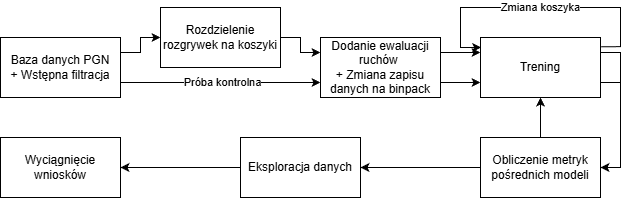
\includegraphics[width=0.7\linewidth]{workflow.png}
    \end{center}
\end{frame}

\begin{frame}{1. Cel Badania}
    \textbf{Badanie zachowania silnika NN podczas uczenia na danych o rosnącym poziomie umiejętności.}
    \vspace{0.5cm}
    \begin{itemize}
        \item Analiza stosunku między Elo danych uczących a Elo powstałego modelu.
        \item Wpływ \textit{curriculum learning} na prędkość nauki i styl gry.
        \item Porównanie modelu badawczego z modelem kontrolnym.
    \end{itemize}
\end{frame}

\begin{frame}{2. Hipotezy}
    \begin{block}{H1: Szybsza nauka cech}
        Model szybciej odnajdzie wzorce, gdyż gracze o niskim Elo kierują się mniej skomplikowanymi przemyśleniami.
    \end{block}
    \begin{block}{H2: Ludzki styl gry}
        Model na każdym etapie będzie grał podobnie do człowieka, unikając losowych ruchów charakterystycznych dla modeli uczonych na wszystkich taktykach naraz.
    \end{block}
    \begin{block}{H3: Korelacja Elo}
        Istnieje ścisła zależność między rankingiem zbioru treningowego a siłą gry modelu końcowego.
    \end{block}
\end{frame}

\begin{frame}{3. Metodologia}
    \begin{itemize}
        \item \textbf{Start:} Wykorzystanie modelu znającego podstawy szachów w celu optymalizacji czasu obliczeń.
        \item \textbf{Dane:} Zbiory pogrupowane w koszyki Elo. Przejście do kolejnego koszyka po określonej liczbie epok lub osiągnięciu progu jakości.
        \item \textbf{Zapis:} Archiwizacja wag modelu po każdej zmianie przedziału.
        \item \textbf{Kontrola:} Równoległy trening modelu na przemieszanym zbiorze danych (bez podziału na rangi).
    \end{itemize}
\end{frame}

\begin{frame}{4. Metryki}
    \begin{columns}
        \column{0.5\textwidth}
        \begin{itemize}
            \item \textbf{Elo:} Turnieje przeciwko silnikom o znanym rankingu.
            \item \textbf{Human-like Index:} Zgodność z ruchami ludzi.
        \end{itemize}
        \column{0.5\textwidth}
        \begin{itemize}
            \item \textbf{Loss Curve:} Analiza funkcji straty przy zmianie koszyka na wyższe Elo.
        \end{itemize}
    \end{columns}
\end{frame}

\begin{frame}{5. Spodziewane Wyniki}
    \begin{center}
        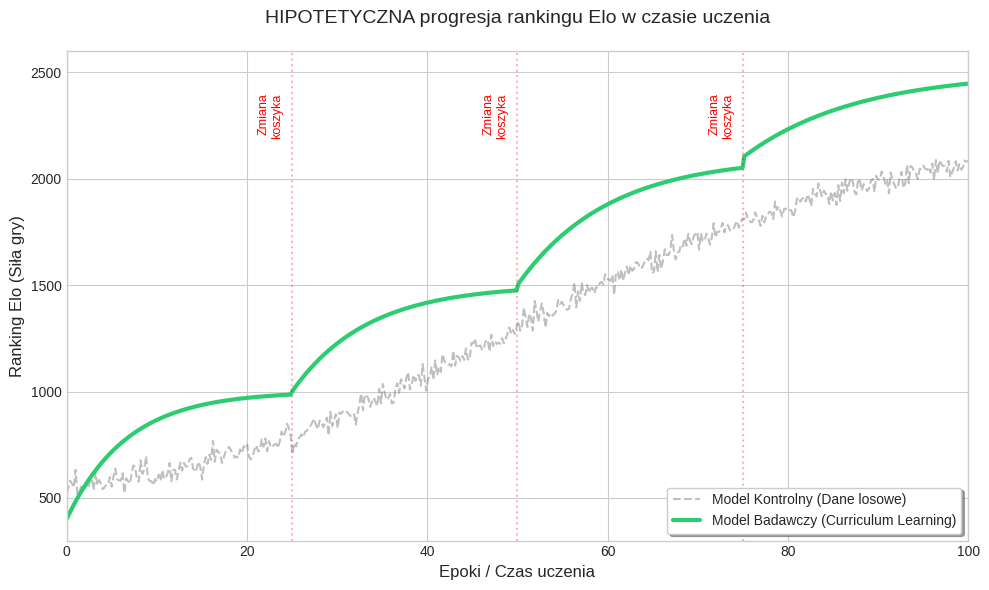
\includegraphics[width=0.7\linewidth]{hypothetical_plot.png}
    \end{center}
    \begin{itemize}
        \item Model badawczy szybciej odnajdzie kluczowe cechy.
        \item Spodziewane "skoki rozwojowe" przy zmianach koszyków.
    \end{itemize}
\end{frame}

\begin{frame}{6. Wnioski i Zastosowanie}
    \begin{itemize}
        \item Weryfikacja akceleracji nauki przez stopniowanie trudności danych.
        \item Ocena przewidywalności modelu dla człowieka.
        \item \textbf{Zastosowanie:} Interaktywny asystent szachowy rozwijający się wraz z użytkownikiem.
    \end{itemize}
\end{frame}

\end{document}